\chapter{Cooper-Paare und Supraleitung\label{chapter:supraleitung}}
\lhead{Cooper-Paare und Supraleitung}
\begin{refsection}
\chapterauthor{Simon Kuster und Nicola Ochsenbein}

%TODO Stichworte einfügen

%----------------------------Einleitung------------------------
In diesem Kapitel m"ochten wir die Grundlagen f"ur das das Kaptiel \ref{chapter:bose} und
die Supraleitung erarbeiten. Im Kaptiel \ref{chapter:bose} werden Elektronen ben"otigt,
die sich wie Bosonen verhalten. Bosonen haben im Gegensatz zu den Elektronen
keinen Spin. Um bei den Elektronen den Spin zu verbergen, eignen sich zwei Elektronen als Paar mit
antiparallelem Spin.

Ausgehend von der bekannten abstossenden coulombschen Wechelwirkung zwischen Elektronen,
wollen wir verstehen, wie und aus welchem Grund sich Elektronen zu Paaren bilden k"onnen,
sogenannten Cooper-Paaren.
Dazu m"ussen wir zuerst den Effekt der Elektron-Elektron Wechselwirkung verstehen.
Aufbauend k"onnen wir dann erkl"aren, welches die energetisch g"unstigsten und somit auch
wahrscheindlichsten Konstellationen sind, unter welchen sich die Elektronen zu Paaren binden.
%TODO Auf Literatur verweisen, wie?

%----------------------------Elektron-Elektron Wechselwirkung------------------------
\section{Elektron-Elektron Wechselwirkung\label{supraleitung:elektronelektronwecheslwirkung}}
\rhead{Elektron-Elektron Wechselwirkung}
Damit sich Elektronen zu Paaren binden, m"ussen sie sich anziehen.
Die bekannte coulombsche Wechselwirkung ist jedoch abstossend.
Dies liegt daran, dass die Ladungen der Elektronen die selben Vorzeichen aufweisen.
\begin{equation}
F = \frac{Q_1\cdot Q_2}{4\pi \varepsilon r^2}
\label{supraleitung:Coulomb}
\end{equation}
Wir sind also auf der Suche nach einer anziehenden Kraft.
Um der Vorzeichenkonvention zu entsprechen muss die Kraft negativ sein.

Zwischen den Elektronen und dem Gitter ist eine Wechselwirkung vorhanden.
Die coulombsche Wechselwirkung zwischen Elektronen und Gitter hat jedoch keinen Einfluss auf die
Elektron-Elektron Wechselwirkung.
Sie wird deshalb nachfolgend nicht ber"ucksichtigt.
Die f"ur uns interessante Elektron-Elektron Wechselwirkung funktioniert "uber die sogenannten Phononen.
Wie diese Wechselwirkung im Allgemeinen funktioniert und was Phononen sind wird nachfolgend erl"autert.

In Abbildung \ref{supraleitung:Gitter} a) betrachten wir einen Ausschnitt der Gitterstruktur eines K"orpers.
Fliegt nun ein Elektron in diesen Gitter-Ausschnitt hinein, so wird das Gitter durch das
elektrische Feld des Elektrons deformiert.
Das Elektron "andert seine Flugbahn.
Dargestellt ist dies in Abbildung \ref{supraleitung:Gitter} b).
Das deformierte Gitter bewegt sich nun weiter als Schwingung.
In Abbildung \ref{supraleitung:Gitter} c) ist diese Schwingung dargestellt und mit $q$ bezeichnet.
Wenn nun ein weiteres Elektron ins Gitter fliegt und auf die Schwingung trifft,
wird dieses von der Schwingung im Gitter beeinflusst, ersichtlich in Abbilung \ref{supraleitung:Gitter} d).
Die Schwingung im Gitter wird wieder vernichtet und das zweite Elektron ver"andert
ebenfalls seine Flugbahn.
Es wurde also ein Impuls $q$ vom Elektron $k'$ zum Elektron $k$ "uber das Gitter transportiert. 

Die Schwingung $q$ welche vom Elektron $k'$ zum Elektron $k$ \glqq transportiert\grqq~wurde
entspricht einem harmonischen Oszillator.
Nach Kapitel \ref{chapter:harmonischeroszillator} bedeuted das, dass die m"oglichen Frequenzen,
und die damit enthaltenen Energieniveaus, quantisiert sind.
Wenn diese Energie quantisiert ist, kann man die Energie der Einfachheit halber als Teilchen betrachten.
Diese neu eingef"uhrten Teilchen werden Phononen genannt.

Um die Darstellung der Wechselwirkung zu vereinfachen, zeichnen wir nun dieses Phonon
als zickzack Vektor zwischen Elektron $k'$ und $k$. Diese Darstellung nach Feynman
ist in Abbildung \ref{supraleitung:FeynmanDiagram1} auf der linken Seite ersichtlich.
Dieser Prozess kann nat"urlich auch umgekehrt vonstatten gehen.
Zuerst wird ein Phonon aufgenommen, danach von einem zweiten Elektron, ein Phonon abgegeben.
Dieser Vorgang ist auf der rechten Seite in Abbildung \ref{supraleitung:FeynmanDiagram1} ersichtlich.

%TODO hier sollte auf das Feynmandiagramm verwiesen werden. (wie?)
%Kann das verhalten der Bilder so beeinflusst werden, dass sie wenigstens im gleichen unterkapitel
%angezeigt werden? (momentan ist die Darstellung der Bilder "uber so viele Seiten nicht geeignet.
\begin{figure} %Feynman Diagram
\centering
\newcommand{\marrow}[5]{%
    \fmfcmd{style_def marrow#1
    expr p = drawarrow subpath (1/4, 3/4) of p shifted 6 #2 withpen pencircle scaled 0.4;
    label.#3(btex #4 etex, point 0.5 of p shifted 6 #2);
    enddef;}
    \fmf{marrow#1,tension=0}{#5}}
\begin{center}
\begin{fmffile}{supraleitung/phonon}
\begin{fmfgraph*}(100,60)
\fmfleftn{i}{2}
\fmfrightn{o}{2}
\fmflabel{$\vec k'-\vec q$}{i1}
\fmflabel{$\vec k'$}{i2}
\fmflabel{$\vec k+\vec q$}{o1}
\fmflabel{$\vec k$}{o2}
\fmf{fermion}{i2,v1,i1}
\fmf{fermion}{o2,v2,o1}
\fmf{zigzag,label=$\vec q$}{v1,v2}
\fmfdot{v1,v2}
\marrow{c}{up}{top}{}{v1,v2}
\end{fmfgraph*}
\qquad
\qquad
\qquad
\begin{fmfgraph*}(100,60)
\fmfleftn{i}{2}
\fmfrightn{o}{2}
\fmflabel{$\vec k'+\vec q$}{i1}
\fmflabel{$\vec k'$}{i2}
\fmflabel{$\vec k-\vec q$}{o1}
\fmflabel{$\vec k$}{o2}
\fmf{fermion}{i2,v1,i1}
\fmf{fermion}{o2,v2,o1}
\fmf{zigzag,label=$-\vec q$}{v1,v2}
\fmfdot{v1,v2}
\marrow{c}{up}{top}{}{v2,v1}
\end{fmfgraph*}
\end{fmffile}
\end{center}

\caption{Entstehung von Cooper-Paaren und Supraleitung nach Feynman \cite{supraleitung:feynman}
\label{supraleitung:FeynmanDiagram1}}
\end{figure}

%-------Gitter Bilder-------
\begin{figure}
\centering
  \begin{tabular}{l l}
  \centering
    \begin{minipage}{0.5\textwidth}
	\includegraphics[width=0.8\textwidth]{supraleitung/gitter-1.pdf}
    \end{minipage}
    &
    \begin{minipage}{0.5\textwidth}
	\includegraphics[width=0.8\textwidth]{supraleitung/gitter-2.pdf}	
    \end{minipage}
    \\
    a)\quad Ungest"ortes Gitter
    &
    b)\quad Elektron fliegt ins Gitter und st"ort dieses
    \\
    \begin{minipage}{0.5\textwidth}
	\includegraphics[width=0.8\textwidth]{supraleitung/gitter-3.pdf}
    \end{minipage}
    &
    \begin{minipage}{0.5\textwidth}
	\includegraphics[width=0.8\textwidth]{supraleitung/gitter-4.pdf}
    \end{minipage}
    \\
    c)\quad Gitter mit Schwingung q
    &
    d)\quad Elektron fliegt ins Gitter und wird beeinflusst
    \\
  \end{tabular}
  \caption{Elektron-Elektron Wechelwirkung mit Gitterdarstellung
  \label{supraleitung:Gitter}}
\end{figure}

%-------Gitter Bilder-------
\begin{figure}
\centering
  \begin{tabular}[b]{l l}
  \centering
    \subfigure[Ungest"ortes Gitter]{\label{supraleitung:Gitter1}
    \includegraphics[width=0.4\textwidth]{supraleitung/gitter-1.pdf}}
    &
    \subfigure[Elektron fliegt ins Gitter und st"ort dieses]{\label{supraleitung:Gitter2}
    \includegraphics[width=0.4\textwidth]{supraleitung/gitter-2.pdf}}
    \\
    \subfigure[Gitter mit Schwingung q]{\label{supraleitung:Gitter3}
    \includegraphics[width=0.4\textwidth]{supraleitung/gitter-3.pdf}}
    &
    \subfigure[Elektron fliegt ins Gitter und wird beeinflusst]{\label{supraleitung:Gitter4}
    \includegraphics[width=0.4\textwidth]{supraleitung/gitter-4.pdf}}
    \\
  \end{tabular}
  \caption{Elektron-Elektron Wechelwirkung mit Gitterdarstellung
  \label{supraleitung:Gitter2}}
\end{figure}

%TODO Bessere Ausrichtung verschiedene Bilderhoehen
%TODO referenzen anpassen

Diese Wechselwirkung zwischen den Elektronen nur grafisch zu betrachten reicht nicht,
um eine Aussage "uber Anziehung oder Abstossung zu machen.
Wir werden also nachfolgend diese Wechselwirkung mathematisch entwickeln.
F"ur die mathematische Betrachtung beginnen wir da, wo wir einen Anhaltspunkt haben, also beim Phonon.

Wir haben gesehen, dass das Phonon einem harmonischen Oszillator entspricht und quantisiert ist.
F"ur das Phonon gibt es also Auf- und Absteigeoperatoren.
Wenn wir die zum Phonon geh"orenden Operatoren $a$ nennen und das Phonon die Energie $q$ hat,
ergibt sich der Aufsteigeoperator
$a^+_q$ und der Absteigeoperator $a_q$.
Da die vom Phonon aufgenommene Energie quantisiert ist, muss das Elektron quantisierte Energie
abgeben und aufnehmen.
Dies bedeuted, dass auch die Elektronen Auf- und Absteigeoperatoren haben.
Wir nennen die zu den Elektronen Operatoren nun $c$. Hat das Elektron die Energie $k$, %TODO Elektronen Operatoren oder Elektronenoperatoren
was der Wellenzahl entspricht, erigbt sich der Aufsteigeoperator $c^+_k$ und der
Absteigeoperator $c_k$ ist.
Zu den entsprechenden Operatoren wird nun also die Energie als Index angegeben.
Wir f"uhren nun noch einen Anfangszustand $|a\rangle$ (vlg. Abb. \ref{supraleitung:Gitter} a)),
einen Endzustand $\langle e|$ (vgl. Abb. \ref{supraleitung:Gitter4}) und
einen Zwischenzustand $z_1$ (vgl. Abb. \ref{supraleitung:Gitter3}) ein.
Der Vorgang der Wechselwirkung zwischen den Elektronen kann nun so beschrieben werden
(ohne Energiebetrachtung):
\begin{equation}
\langle e|c^+_{k+q} c_k a_q |z_1\rangle\langle z_1| c^+_{k'-q} c_{k'} a^+_q |a\rangle
\label{supraleitung:WechelwirkungOE}
\end{equation}
Zu beachten ist dabei, dass die Leserichtung von rechts nach links ist.
Es wird also vom Anfangszustand aus ein Phonon $a_q$ erzeugt, ein Elektron $c_{k'}$ vernichtet
und ein Elektron $c_{k'+q}$ erzeugt, um zum Zwischenzustand $z_1$ zu gelangen.
Von diesem Zwischenzustand aus geht es weiter, indem man das Phonon $a_q$ wieder vernichtet,
das Elektron $c_k$ vernichtet und ein Elektron $c_{k+q}$ erzeugt.

Als n"achstes m"ussen wir die Energiebetrachtung einf"ugen.
Daf"ur f"uhren wir eine materialabh"angige Konstante $M_q$ ein und erg"anzen die
Wechselwirkung mit dem Nenner aus der St"orungstheorie.
Um die gesammte Wechselwirkung zu erhalten summieren wir "uber alle $k$, $k'$ und $q$.
Die Wechselwirkung erg"anzen wir zudem um einen zweiten Term der die umgekehrte
Wechselwirkungs-Reihenfolge enth"alt.
Dies f"uhrt dazu, dass wir sp"ater weitere Vereifachungen durchf"uhren k"onnen.
Da wir aber nun die Wechselwirkung doppelt z"ahlen (wir summieren ja bereits "uber alles)
teilen wir noch durch $2$.

\begin{equation}
H_{\text{pair}}=
\frac{1}{2}
\sum \limits_{kk'q} |M_q|^2
\left\{
\frac
{\langle e|c^+_{k+q} c_k a_q |z_1\rangle\langle z_1| c^+_{k'-q} c_{k'} a^+_q |a\rangle }
{E(k')-E(k'-q)-\hbar\omega_q}
+
\frac
{\langle e|c^+_{k'-q} c_{k'} a_{-q}|z_1\rangle\langle z_1| c^+_{k+q} c_k a^+_{-q} |a\rangle }
{E(k)-E(k+q)-\hbar\omega_q}
\right\}
\label{supraleitung:WechelwirkungME}
\end{equation}

Die Energieerhaltung muss hier erf"ullt sein. Dies erlaubt uns folgende Vereinfachung zu machen:
$E(k')-E(k'-q) = E(k+q)-E(k)$. Wir ersetzen $E(k')-E(k'-q)$ durch $E(k+q)-E(k)$.
Zus"atzlich k"urzen wir die Phononen und den Zwischenzustand und packen
alles ausser der reinen Wechselwirkung in einen Koeffitienten $V_{kk'q}$.
Wir sehen nun zwar den inneren Ablauf des Prozesses nicht mehr, daf"ur kann die Formel
weiter vereinfacht werden.
Wir erhalten die Formel:
\begin{equation}
H_{\text{pair}}=
\frac{1}{2}
\sum \limits_{kk'q} 
\langle e|V_{kk'q}c^+_{k+q}c^+_{k'-q}c_{k'}c_k|a \rangle
\label{supraleitung:WechelwirkungKurz}
\end{equation}
mit
\begin{equation}
V_{kk'q} = - |M_q|^2 \left\{
\frac{1}{\hbar\omega_q-(E(k+q)-E(k))}
+
\frac{1}{\hbar\omega_q+(E(k+q)-E(k))}
\right\}
\label{supraleitung:WechelwirkungVkk'q}
\end{equation}
Wir vereinfachen weiter mit $(a-b)\cdot (a+b) = a^2-b^2$.

\begin{equation}
V_{kk'q} =
\frac
{2|M_q|^2\hbar\omega_q}
{(E(k+q)-E(k))^2-(\hbar\omega_q)^2}
\label{supraleitung:Wechelwirkung_Vkk'q_Kurz}
\end{equation}
Das Vorzeichen von $V_{kk'q}$ entscheidet nun dar"uber, ob die Wechselwirkung
anziehend oder abstossend ist.

Da der Z"ahler positiv ist, wird das Vorzeichen von $(E(k+q)-E(k))^2-(\hbar\omega_q)^2$ bestimmt.

%----------------------------Hinzufuegen von Elektronen zu der Fermikugel------------------------
\section{Hinzuf"ugen von Elektronen zu der Fermikugel}
\rhead{Hinzuf"ugen von Elektronen zu der Fermikugel}
Angenommen, solch eine Elektron-Elektron Wechselwirkung, wie im Kapitel
\ref{supraleitung:elektronelektronwecheslwirkung} beschrieben, kommt zustande,
wollen wir nachfolgend herausfinden, welche Bedingungen erf"ullt sein m"ussen.

Unser Ziel wird nun sein, zwei Elektronen energetisch m"oglichst g"unstig zur Fermikugel hinzuzuf"ugen.
Dazu ben"otigen wir die theoretischen Grundlagen zur Fermikugel welche im Kapitel
\ref{chapter:festkoerper} behandelt sind.


Die Wechselwirkung zwischen den Elektronen besteht einerseits aus der altbekannten coulombschen
Wechselwirkung (vgl. Gl. \ref{supraleitung:Coulomb}) und der neu eingef"uhrten
Elektronen-Elektronen Wechselwirkung.
Welche dieser Kr"afte "uberwiegt, entscheidet die St"arke der Elektronen-Phononen-Kopplung.

\index{Elektronengas}
Um diese neue Wechselwirkung zu betrachten, gehen wir von einem idealisierten Falls aus.
Dazu kann das Modell des Elektronengases verwendet werden.
Dabei sind die Valenzelektronen nicht an die einzelnen Gitterpl"atze der Atome gebunden sondern k"onnen sich,
wie in einem klassischen Gas, frei bewegen.
Diese freien Elektronen sind verantwortlich f"ur die Leitf"ahigkeit von Metallen.
Dieses Modell kann auch auf ein sehr stark gek"uhlter metallischer K"orper angewendet werden,
was f"ur die Supraleitung von Bedeutung ist.
%TODO Abschnitt ueberpruefen

Wir betrachten die Fermikugel in der $k$-Ebene, in welcher alle inneren Zust"ande besetzt sind,
alle "ausseren Zust"ande seien frei.
Zu diesem System werden nun zwei Elektronen $(k_1,E(k_1))$ und $(k_2,E(k_2))$ hinzugef"ugt.
Wir beschr"anken uns auf die Wechselwirkungen in welchen keine Energie an das Atomgitter abgegeben wird.
Zudem beschr"anken wird die maximal zul"assige Wechselwirkung zwischen den Elektronen auf die
Energie eines Phonons.

\begin{equation}
|E(k+q)-E(k)|\le\hbar\omega_q
\label{supraleitung:Phonon Energie}
\end{equation}

Ist diese Bedingung erf"ullt, wird das Vorzeichen in der Gleichung \ref{supraleitung:Wechelwirkung_Vkk'q_Kurz} negativ und die Elektron-Elektron Wechselwirkung wird anziehend.

\subsubsection{Wellenfunktion}
\rhead{Wellenfunktion}
Die Wellenfunktion des Elektronenpaares wird durch die Anwendung zweier Aufsteigeoperatoren
auf den Grundzustand $|G\rangle$ der gef"ullten Fermikugel aufgebaut, indem wir "uber
alle m"oglichen Wellenzahlvektoren $k_1$ und $k_2$ $(|k_i| \ge k_f)$ und "uber
die Elektronenspins $\sigma_1$ und $\sigma_2$ summieren.
$a$ stellt den Fourierkoeffizienten des jeweiligen Summanden dar.

\begin{equation}
\Psi_{12}=\sum \limits_{k_1k_2\sigma_1\sigma_2} a_{\sigma_1\sigma_2}
(k_1,k_2)c^+_{k_1\sigma_1}c^+_{k_2\sigma_2}|G\rangle
\label{supraleitung:WellenfktAllg}
\end{equation}

Um einen Zustand mit definiertem Gesamtimpuls zu erhalten, f"uhren wir die Summation in
(\ref{supraleitung:WellenfktAllg}) unter der Nebenbedingung $K=k_1+k_2=\texttt{const}$ aus.
Zus"atzlich fordern wir, dass eine Wechselwirkung zwischen den Elektronen nur dann bestehen soll,
wenn sich ihre Zust"ande ausserhalb der Fermikugel mit der Energie
$(E_F \le E(k_i) \le E_F+\hbar\omega_q)$ befinden.
Zusammengefasst ergeben sich folgende drei Bedingungen:
\[
\overrightarrow{k_1}+\overrightarrow{k_2}=\overrightarrow{K}=const
\]
\[
E_F\le|\overrightarrow{k_1}|\le E_F+\hbar\omega_q
\]
\[
E_F\le|\overrightarrow{k_2}|\le E_F+\hbar\omega_q
\]
\subsubsection{Optimaler Gesamtimpuls von $k_1$ und $k_2$ finden}
\rhead{Optimaler Gesamtimpuls von k1 und k2 finden}

Die Wechselwirkungsenergie wird umso gr"osser, je mehr Summationsglieder zur Wellenfunktion
(\ref{supraleitung:WellenfktAllg}) beitragen.
Der Gesamtimpuls $K$ soll nun also so bestimmen werden, dass die Wechselwirkungsenergie maximal wird.

Zur Bestimmung des optimalen $K$ kann die Fermikugel mit einer Schale der Dicke
$\hbar\omega_q$ im $k$-Raum aufgezeichnet werden.
In der Abbildung \ref{supraleitung:kRaum} a) wurde ein beliebiges $K$ gew"ahlt und durch
geometrische Konstruktion gezeigt, in welchen Bereichen (grau markiert) m"ogliche $k_1$ und $k_2$
gew"ahlt werden k"onnen.
Die graue Fl"ache entspricht der Wahrscheinlichkeit, denn je mehr M"oglichkeiten f"ur die Wahl
von $k_1$ und $k_2$ vorhanden sind, desto gr"osser ist die Wahrscheinlichkeit und entsprechend
die graue Fl"ache.
Ist $K$ gr"osser als $2\cdot(E_F+\hbar\omega_q)$ k"onnen keine g"ultigen L"osungen mehr
f"ur $k_1$ und $k_2$ gefunden werden (Abbildung \ref{supraleitung:kRaum} b)).
W"ahlt man hingegen $K$ kleiner und im Extremfall $K=0$, erzielt man die gr"osst m"ogliche
Fl"ache und entsprechend die gr"osste Wahrscheinlichkeit (Abbildung \ref{supraleitung:kRaum} c)).
Man findet so heraus, dass die Wahrschinlichkeit am gr"ossten ist, wenn die
Wellenzahlvektoren $k_1$ und $k_2$ entgegengesetzt sind.

% Visualisierung der besten K-Vektors
\begin{figure}
\centering
  \begin{tabular}{l l l}
  \centering
    &
    \begin{minipage}{0.6\textwidth}
	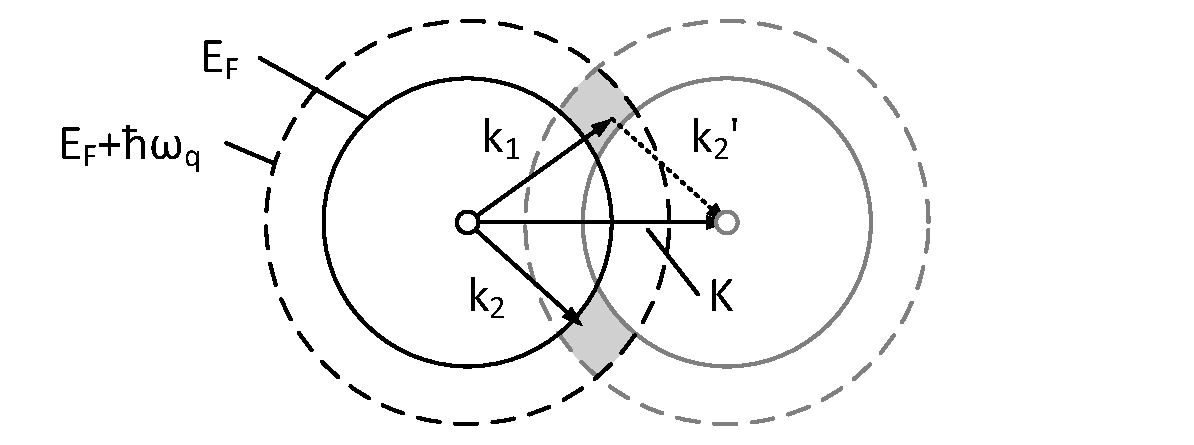
\includegraphics[width=1.2\textwidth]{supraleitung/Graphics/kGraphic05g.pdf}
    \end{minipage}
    &
    \\
    &
    a)\quad beliebiges K gew"ahlt 			%K gr"osser 0, kleiner Ef+hwq, mit Fl"achenmarkierung
    \\
    &
    \\
    &
    \begin{minipage}{0.6\textwidth}
	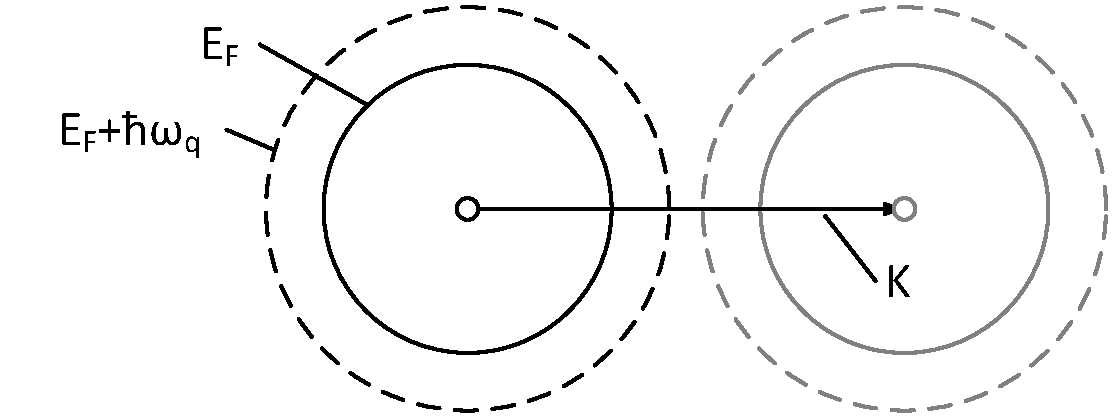
\includegraphics[width=1.2\textwidth]{supraleitung/Graphics/kGraphic06g.pdf} 
    \end{minipage}
    &
    \\
    &
    b)\quad K zu gross grw"ahlt							%K zu gross
    \\
    &
    \\
    &
    \begin{minipage}{0.6\textwidth}
	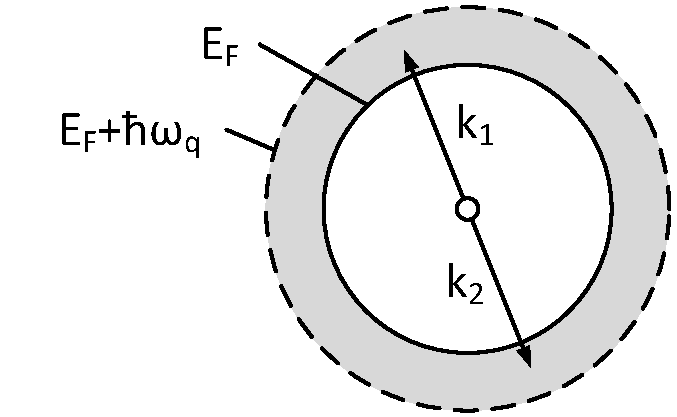
\includegraphics[width=1.2\textwidth]{supraleitung/Graphics/kGraphic09g.pdf}
    \end{minipage}
    &
    \\
    &
    c)\quad Maximale Anzahl M"oglichkeiten um $k_1$, $k_2$ zu w"ahlen mit K = 0 	%K gleich 0, mit Fl"achenmarkierung
    &
    \\
  \end{tabular}
  \caption{Visualisierung des Gesamtimpulses im $k$-Raum
  \label{supraleitung:kRaum}}
\end{figure}

\subsubsection{Spin}
\rhead{Spin}
Bekanntlich besitzen Elektronen einen Spin.
Da wir auf der Suche nach der maximalen anziehenden Wechselwirkung sind, nehmen wir an,
dass die Elektronenspins antiparallel sind.
Hierzu kann die "Uberlegung mit dem entstehenden magnetischen Feld herbeigezogen werden.
W"aren die Elektronenspin parallel w"urden sich die entstehenden magnetischen Felder abstossen.
Wobei hingegen bei antiparallelem Elektronenspin die Wechselwirkungsenergie durch die
anziehenden magnetischen Felder verst"arkt wird.

\subsubsection{Neue Wellenfunktion}
\rhead{Neue Wellenfunktion}
Mit den gewonnenen Erkenntnissen, dass der Gesamtimpuls $K=0$ ist und die Elektronenspin
\texttt{antiparallel} sind, ergibt sich die vereinfachte Wellenfunktion

\[
\Psi_{12}=\sum \limits_{k} a(k)c^+_{k}c^+_{-k}|G\rangle.
\]

Um eine kompakte Schreibweise zu erhalten ordnen wir $k$ zugleich \glqq Spin
aufw"arts\grqq~und $-k$ \glqq Spin abw"arts\grqq~zu.
Der g"unstigste Prozess ist also, wenn die Elektronen entgegengesetzte
Wellenzahlvektoren $(k_1 = -k_2)$ und entgegengesetzten Spin $(\sigma_1 = -\sigma_2)$ aufweisen.

\section{Ausblick}
\rhead{Ausblick}
Wir haben also gesehen, dass es eine Elektron-Elektron Wechselwirkung gibt und wie diese zustande kommt.
Das Vorzeichen und somit die Cooper-Paar Bildung sind aber noch nicht gekl"art.
Um das Vorzeichen zu berechnen sind weitere Vereinfachungen zu treffen.
Man erh"alt dann eine Gleichung mit einer zu minimierenden Nebenbedingung.
Durch weitere Approximationen findet man heraus,
dass 2 Elektronen als Paar weniger Energie ben"otigen, als wenn man sie einzeln zur Fermikugel
hinzuf"ugen w"urde.
F"ur die Berechnung und als weiterf"uhrende Literatur verweisen wir auf
O. Madelung Festk"orper II (\cite{supraleitung:madelung1}).


\printbibliography[heading=subbibliography]
\end{refsection}



